\documentclass[12pt]{article}
\usepackage{amsmath, amsfonts, tikz}
\usetikzlibrary{arrows.meta}

\definecolor{lightA}{RGB}{187, 221, 249}
\definecolor{darkA} {RGB}{8,   120, 211}
\definecolor{lightB}{RGB}{204, 140, 242}
\definecolor{darkB} {RGB}{125,   3, 196}

\newcommand{\R}{\mathbb{R}}

\begin{document}
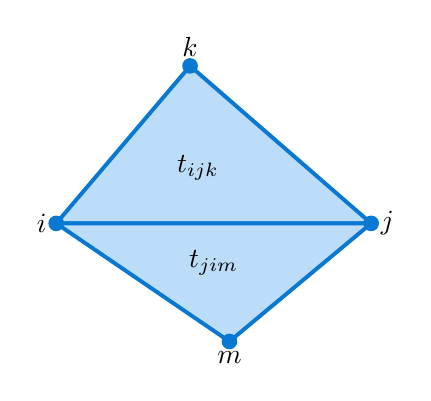
\begin{tikzpicture}
  \coordinate (A) at (0,0);
  \coordinate (B) at (4,0);
  \coordinate (C) at (1.7, 2);
  \coordinate (D) at (2.2, -1.5);

  \node[anchor=east]  at (A) {$i$};
  \node[anchor=west]  at (B) {$j$};
  \node[anchor=south] at (C) {$k$};
  \node[anchor=north] at (D) {$m$};

  \path[draw, color=darkA, fill=lightA, line width=0.5mm, line cap=round] (A) -- (B) -- (C) -- cycle;
  \path[draw, color=darkA, fill=lightA, line width=0.5mm, line cap=round] (A) -- (B) -- (D) -- cycle;

  \node[circle, fill=darkA, inner sep=2pt] at (A) {};
  \node[circle, fill=darkA, inner sep=2pt] at (B) {};
  \node[circle, fill=darkA, inner sep=2pt] at (C) {};
  \node[circle, fill=darkA, inner sep=2pt] at (D) {};

  \node at (1.8, 0.7) {$t_{ijk}$};
  \node at (2, -0.5) {$t_{jim}$};
\end{tikzpicture}

\vspace{5mm}

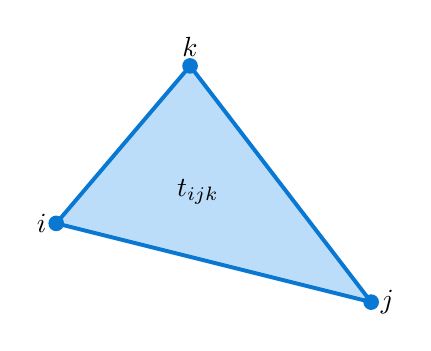
\begin{tikzpicture}
  \coordinate (A) at (0,0);
  \coordinate (B) at (4,-1);
  \coordinate (C) at (1.7, 2);

  \node[anchor=east]  at (A) {$i$};
  \node[anchor=west]  at (B) {$j$};
  \node[anchor=south] at (C) {$k$};

  \path[draw, color=darkA, fill=lightA, line width=0.5mm, line cap=round] (A) -- (B) -- (C) -- cycle;

  \node[circle, fill=darkA, inner sep=2pt] at (A) {};
  \node[circle, fill=darkA, inner sep=2pt] at (B) {};
  \node[circle, fill=darkA, inner sep=2pt] at (C) {};

  \node at (1.8, 0.4) {$t_{ijk}$};
\end{tikzpicture}

\end{document}
